Within this paper, we will restrict our attention to cases where there is a
decision problem under scrutiny that can be formulated as follows: There is a
population of individual $I = \{i_1, i_2, \dots, i_n\}$ over whom we must
distribute a resource $R$. Following \cite{Kuppler_2021}, we define a
\emph{decision rule} as a mapping $d: I \to \{0, 1\}$ which determines whether
or not a given individual $i_n$ receives an amount of resource $R$. An
algorithmic deicion-maker on this account is a decision rule $d$ which is
implemented by an algorithm.

At this time, it worth defining what we mean by a resource $R$ more carefully.
For this purpose, we will use Rawls' definition of a primary
good~\cite{Rawls_1971}. For Rawls, these are a specific category of goods which
consist of 
\begin{enumerate}
    \item Basic rights and liberties
    \item Freedom of movement and free choice among a wide range of occupations
    \item Powers of office and positions of responsibility
    \item Income and wealth
\end{enumerate}
For our purposes, any such primary good is fit to be considered a resource
in our decision problem. The typical problem domains for algorithmic
fairness fit neatly within these categories. For example, college admissions
algorithms adjudicate freedom of occupation, bank loan algorithms distribute
wealth, promotion algorithms in the worksplace divy up positions of
responsibility, and prison parole decisions determine freedom of movement.

Admittedly, not all problem domains in which algorithmic decision-making is
applied can be formulated in this way~\cite{Green_2017}. For example,
applications of AI in natural language translation may not be easily formulated
in terms of resource allocation, but the reader may still be concerned with the
perpetuation of social biases through the decisions it makes in translation.
While these cases are significant, they do not fall simply within the domain of
distributive justice, and so we will not consider them here.

\subsection{Algorithmic Fairness Measures}\label{sec:fairness-measures}
In the typical presentation of algorithmic fairness, we are given a population
of individuals $I = \{i_1, i_2, \ldots, i_n\}$ who have a set of covariates
$P$. There are a set of morally protected covariates, $M \subseteq P$ of an
individual, an observed set of covariates $X \subseteq P$ for each individual,
and therefore a set of observed morally protected covariates $A = X \cap M$.

Our algorithm is a classification function $f: X \to {0, 1}$ mapping covariates
of each individual to a binary outcome~\cite{CorbettDavies_2023}. A fairness
metric is a function over $f$ and $A$ designed to measure the extent to which
$f$ obeys some constraint on the distribution of outcomes with respect to $A$.

With respect to the decision problem described above, we now have a model for 
the full decision-making process. For each individual competing for a resource,
we have a decision rule which says to measure a set of covariates $X$ for each
individual, and then apply $f$ to $X$ to determine whether or not to allocate
$R$ to that individual.

Note the strict difference between the decision rule $d$ and the function $f$.
The decision rule operates on the entire individual $i_n$, while the
classification function operates only on the observed covariates from the
individual. This distinction is important because it demonstrates a key
limitation of algorithmic fairness measures. One might be concerned that a
decision rule is unfair despite a fair classification function if the covariates
input into the classifcation function are not a complete or accurate
representation of the individual.

As a running example, consider the case of a hiring algorithm. The decision
problem is to map a set of applicants to hiring decision. Our algorithm must
implement a function to do so based only on the personal information presented
in their resumes, which is their education, experience, race, and gender. We
want to ensure that our hiring practices are fair with respect to race, and
gender. This gives us the following setup:
\begin{center}
    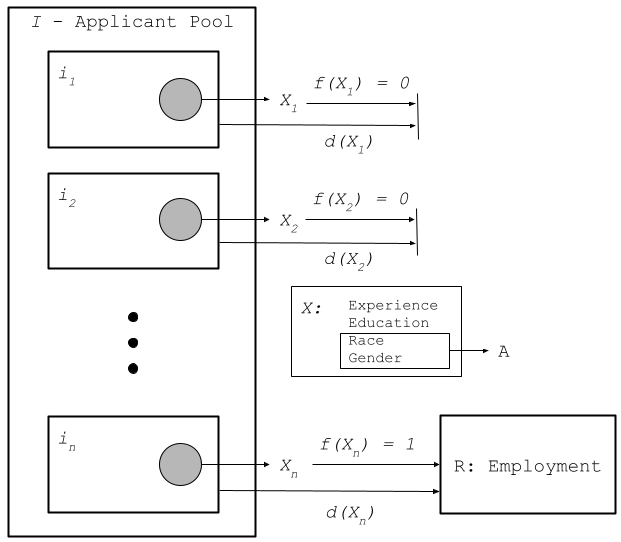
\includegraphics[scale=.4]{figs/fig1.png}\\
    \emph{Fig. 1: A hiring decision algorithm as a decision problem}\\
\end{center}
where a fairness measure will operate exclusively on the mapping from
experience, education, race, and gender to hiring decisions. Whether or not
these factors are a good reputation of the applicants is left unaddressed by
the fairness measure.

Some of the most commonly discussed measures in the literature are presented
below together with their strengths critiques leveraging this lens. For a more
exhaustive list of measures, see~\cite{CorbettDavies_2023}.

\begin{definition}
    Fairness Through Unawarenss — $f$ satisfies fairness through unawareness iff
    \[A = \emptyset\]
\end{definition}

In other words, the classification function may not receive any morally
protected covariates as inputs. So, for our hiring admissions case, we would be
forced to remove race and gender from $X$ and only consider education and
experience.

This notion is intuitively appealing — how can the algorithm dicriminate against
me based on my race if it doesn't know my race? However, it is clear that this
measure is not sufficient to ensure fairness. For example, if I attended a
historically black college, my education may function as a proxy for my race, 
allowing bias to remain in the algorithm.

\begin{definition}
    Demographic Parity — $f$ satisfies demographic parity iff
    \[P[f(X) = 1 | A = a] = P[f(X) = 1]\;\forall a \in A\]~\cite{Dwork_2012}.
\end{definition}

Demographic parity holds that the probability of a positive output ($f(X) = 1$)
should be statistically independent of the protected attributes. This is 
an easily understandable and measurable criteria for fairness. At a first look,
it is appealing — the same number of individuals from each race will be
successful in seeking jobs at a particular company. However, a close look
reveals difficulties.

Under demographic parity, we must balance the probability of success between
groups, which becomes very difficult when the base rates of success are
unequal. For example, if women are much more qualified for a job on average than
men, then demographic parity will require that we hire less qualified men in
place of more qualified women in order to balance the probability of success
between gender groups. In other words, my false positive rate will be very high
for men while my false negative rate will be very high for women, creating a 
severely unfair practice~\cite{Barocas_2017}.

\begin{definition}
    Equalized Odds — $f$ satisfies equalized odds if given true outcomes $D$
    over all individuals, we have
    \[P[Y=1|A=a, D=1] = P[Y=1|A=b, D=1]\;\forall a, b\in A\]
    \[P[Y=1|A=a, D=0] = P[Y=1|A=b, D=0]\;\forall a, b\in A\]~\cite{Hardt_2016}.
\end{definition}

Equalized odds requires that the true positive and false positive rates be
balanced between groups. This is often thought to ensure there is no disparate 
mistreatment across groups. In our hirign case, for example, equalized odds
ensures that no one racial group more likely to be falsely rejected or
erroneously hired than another. If I am rejected from a position despite being
qualified, I can be assured that had my race been different, the probability of
this outcome would have been the same. 

Equalized odds is often critiqued for struggling to deal with unequal base rates
between groups. Consider the following example from criminal justice. We have a 
distribution rule which says to allocate a parole to a prisoner if they are very
unlikely to recidivate. Due to a history of discriminatory practices and social
marginalization, black prisoners have a base rate of recidivism much higher than
white defendants~\cite{CrimeJustice_2023}. As a result, allocating a parole to 
a white prisoner has a base line lower likelihood of being a false positive. 
Therefore, one could achieve equal false positive rates by \textit{adding} false
positives to the white portion of the dataset, resulting in an increase in the
number of white prisoners receiving parole undeservingly. This was exactly the
case in the COMPAS algorithm~\cite{Angwin_2016}. COMPAS was calibrated to have
equal predictive accuracy across racial groups, but this resulted in a higher
false positive rate for black defendants and a much lower false positive rate
for white defendants due to unequal base rates.

\begin{definition}
    Counterfactual Fairness — $f$ satisfies counterfactual fairness iff
    \[P[f(X) = 1 | do(A = a)] = P[f(X) = 1 | do(A = b)]\;\forall a,
                                                   b \in A\]~\cite{Kusner_2018}.
    Where the $do$ operator denotes an intervention on the variable $A$.
\end{definition}

Borrowing from the language of causal inference, counterfactual fairness posits
that the protected attributes may not have any causal effect on the outcome of
te classification function. This is a highly appealing notion of fairness.
If my protected characteristics do not in any way cause the outcome of the
decision rule, then it is difficult to argue that I have been discriminated
against. However, this measure is difficult to implement in practice.

Counterfactual fairness is often critiqued based on the difficulty and potential
subjectivity of detecting causal links between variables. Recent work on the 
social construction of demographic variables reveals that causal modeling may 
have an inherently normative basis~\cite{Hu_Forthcoming}, and even if these
issues are set aside, the computational expense of causal discovery can create
issues of practicality.

This discussion of dominant algorithmic fairness measures and their critiques
reveal that there is no one-size-fits-all solution to the problem of algorithmic
fairness. Each measure has its own strengths and weaknesses, and the choice of
measure will depend on the specific context in which the algorithm is being
applied. However, how should one select a measure? What are the normative
considerations that should guide this choice? In hopes of developing a more
nuanced and structured approach to these questions, we turn to work in the 
philosophy of distributive justice.

\subsection{Theories of Distributive Justice}

Within the formalism we have presented, the role of a theory of distributive
justice is to define what constitutes a fair distribution rule. While 
algorithmic fairness measures operate on the classification function which is
one component of the decision rule, distributive justice operates at one level
higher, defining the rule decision rule in which the classification function is
embedded.

Decision rules posited by theories of distributive justice take on the following
general form: Allocate $R$ to $i_n$ iff $i_n$ has property $y$. Several
conventional theories of distributive justice have been proposed in the
literature, and we will discuss those which have been previously proposed to be
implemented by algorithmic fairness measures here. For a more exhaustive list of
theories available, see~\cite{Kuppler_2021}.

\begin{definition}
    Liberal Egalitarianism — liberal egalitarianism posits that equal stocks of
    resources should be maintained across society~\cite{Rawls_1971}.
\end{definition}

Equally restated in the formalism we have presented, egalitarianism posits that
$R$ should be allocated to $i_n$ iff doing so minimizes the overall inequality
across stocks in the population. Thus in this case, $y$ is the property of
\textit{lacking} $R$ relative to the population. This approach is appealing in
its simplicity and clarity, and in its ability to ensure that all individuals
have access to the same resources.

Note that the precise currency of liberal egalitarianism is unclear. For
example, allocating money to an individual who is lacking in food only
indirectly impacts the stock of concern, but it is clear that doing so will
still reduce the overall inequality of the population. Clearly in this case we
could shift our currency to general wealth or utility, but the choice of
currency is not immediately obvious, nor does it seem generally possible to
define a currency which is globally applicable~\cite{Binns_2018}.

\begin{definition}
    Luck Egalitarianism — Luck egalitarianism posits that individuals should
    receive resources in proportion to their choices and actions, but equally
    with respect to their features which are outside of their
    control~\cite{Knight_2013}.
\end{definition}

Luck egalitarianism posits that $R$ should be allocated to $i_n$ iff $i_n$
deserves $R$ based on some set of their choices and actions which do not include
features outside of their control. This approach is appealing on the grounds of
personal responsibility and autonomy. If I make choices which result in my own
deprivation of $R$, then I am responsible for that deprivation. However, I
cannot be deprived of $R$ on the grounds of features I do not control, such as
my race, gender, or talent.

Luck egalitarianism is often critiqued for being highly subjective and difficult
to measure. What constitutes a choice or action is not always clear, and the
line between what is and is not within an individual's control is often blurry.
Establishing responsibility is already a difficult task in legal philosophy, and
operationalizing this theory in practice is likely to be fraught with
difficulties.

\begin{definition}
    Sufficientarianism — Sufficientarianism posits that all individuals should
    receive a share of resources sufficient to meet some threshold level of
    well-being~\cite{Sen_1979}.
\end{definition}

Sufficientarianism is a theory of distributive justice which posits that the
distribution rule should be such that all agents receive an amount of $R$ which
is sufficient to meet some threshold level of well-being. Thus $y$ is defined as
the property of \textit{needing} $R$. This sort of approach protects the most
vulnerable members of society and ensures that all individuals have access to
the basic goods they need to survive.

Note that what constitutes a threshold level of well-being and what goods are
required for it is not immediately clear, and that under conditions of scarcity
it may be impossible to meet the threshold for all agents. It therefore remains
unclear how to operationalize this theory in practice in many cases.

\begin{definition}
    Moral dessert holds that individuals should receive resources in proportion
    to their moral merit~\cite{Pojman_1997}.
\end{definition}

Theories of dessert therefore set $y$ to be some operationalization of moral
merit. Under the right definition of moral merit, this approach shows promise — 
it is intuitive that someone who has worked hard and done good works across
society deserves reimbursement or insurance of positive outcomes. However,
theories of dessert have been critiqued for being highly subjective and
difficult to measure. Any attempt to craft a metric for moral merit is likely to
be highly controversial and may be subject to manipulation by those in power. 

The main differentiating factor between these theories is the property $y$ which
they posit as the basis for the decision rule. In seeking to understand
algorithmic fairness through the lens of theories of distributive justice, we 
must therefore ask how, if at all, the fairness measures we have presented place
constraints on the property $y$ of the decision rule. Especially given
that the fairness measures operate on the cliassification function which is a
component of the decison rule, to what extent are they capable of enforcing
constraints over the full decision rule? So far as they do enforce constraints
on $y$, how well do they capture the constraints actually posited by the common
theories of distributive justice enumerated here?

\subsection{Relating Algorithmic Fairness to Distributive Justice}

We have now developed the key components of our formalism needed to connect 
algorithmic fairness to theories of distributive justice. In the algorithmic
decision-making process, we have a decision rule which is composed of the
observation of a set of covariates $X$ for each individual, the application
of a classification function to $X$ to determine whether or not to allocate a
resource to that individual, and the allocation of the resource to an individual
if it is dictated by the classification function. Theories of distributive
justice define what a fair decision rule is, and in doing so, they define the
property $y$ which determines whether or not an individual should receive the
resource. Algorithmic fairness measures, on the other hand, operate only on the
classification function. Therefore, it doesn't make sense to argue that an
algorithmic fairness measure directly implements a theory of distributive
justice. Instead, we must evaluate the entire decision rule, including the
mapping from each individual to their observed covariates to determine whether
or not the correct constraints are being placed on $y$ for a given decision
rule.

As a concrete example, return to the case of a hiring algorithm. If $X$ is
modified to exclude education and experience, and to include, say, enjoyment of
Mexican food, then regardless of what fairness measure is satisfied by $f$, $d$
will clearly be unjust according to any theory of distributive justice. This
example demonstrates that the constraints placed on $f$ by a fairness measure
are not sufficient to ensure that the full decision rule $d$ is complies with a
theory of distributive justice, but must operate in conjunction with the
constraints placed on $X$.

Once granted an appropriate $X$ as input to $f$, the role of $f$ becomes to
predict the $y$ desired by the chosen theory of distributive justice. The role
of the fairness measure is then to measure the extent to which $f$ is successful
in doing so. For example, if we are operating under a theory of desert, then
$f$ should predict the moral merit of each individual, and the fairness measure
should measure the extent to which $f$ is successful in doing so. If $f$ is
successful in predicting moral merit, then the decision rule $d$ will be fair
according to the theory of desert. Let us then briefly examine the fairness
measures we have discussed in this light, to see what constraints they place on
$y$ given an appropriate set of observed covariates as input.

\begin{itemize}
    \item Fairness Through Unawareness: Fairness through unawareness places no
        constraints on $y$. It only requires that the classification function
        not receive any morally protected covariates as input. Since morally
        protected covariates can be derived from those covariates which are not
        protected, this measure is essnetially vacuous with respect to the full
        decision rule.
    \item Demographic Parity: Demographic parity mandates that $y$ should not
        deppend on the morally protected covariates. This is too weak a
        constraint to fully implement any theory of distributive justice. For
        example, this condition is \textit{necessary} but not
        \textit{sufficient} for liberal egalitarianism, luck egalitarianism, and
        sufficientarianism, but is not strong enough to fully enforce any of
        these theories.
    \item Equalized Odds: Equalized odds dictates that $y$ should not depend on
        the morally protected covariates given the true outcomes. In other
        words, $y$ is a property of deservingness which is independent of the
        morally protected covariates. This \textit{could} implement moral
        dessert under a particular definition of moral merit in which the
        morally protected covariates are excluded from the operationalization of
        moral merit and the true outcomes are the direct result of moral merit.
        However, this is undesireably working backwards from the fairness
        measure to the theory of distributive justice.
    \item Counterfactual Fairness: Counterfactual fairness requires that $y$ is
        a property of deservingness which is causally independent of the
        morally protected covariates. This measure again implements moral
        dessert under a hyper-specific operationalization that is unproductive
        for our purposes.
\end{itemize}

This analysis reveals that the fairness measures we have discussed are not
sufficient to enforce theories of distributive justice. They place constraints
on the classification function which are too weak to fully enforce the
constraints placed on the full decision rule by theories of distributive
justice, except in hyper-specific cases which are unproductive for justifying 
the use of the fairness measure. What's missing in each case is \textit{detail}:
How does an algorithmic fairness measure enforce the normative contraints about
how $y$ is derived from $X$? This suggests a new account is needed to synthesize
these two fields and to provide a more nuanced and structured approach to
connecting algorithmic fairness to theories of distributive justice. In the
following sections, we will develop such an account through the lens entitlement
justice, which has been largely overlooked in the literature on algorithmic
fairness.
